\section{CAnalytics v2: supporting collaborative hypothesis development}

Based on feedback from study one, we developed CAnalytics V2 and made several improvements. A major change is to enable a structured approach to hypothesis development, as described in Section~\ref{feature-hypothesis}. We developed a hypothesis development panel. When the user creates a hypothesis,
the current state of views are automatically captured, saved and bound to
the hypothesis. Each hypothesis includes a statement as well as a link to the view.
The view includes the data, the filters applied to the data, as well as state of
the visualization, including the zoom level, element positions, graph window size, etc. The exact view could be restored to what it was like when the
hypothesis was created. The hypothesis is shared with the team immediately.
Teammates could ``clone'' the view and use it as a context to understand and further investigate the source hypothesis. Since the view is interactive rather than a static screenshot, collaborators can apply new filters or pivot a different focus, and develop a new hypothesis,
whether supporting or refuting the original one. The system builds a thread structure based
on how the view is ``inherited''. For example, if the view used in
Hypothesis A is re-arranged on the base of the ``clone'' of the view from Hypothesis B, A and B
are in the same hypothesis thread. However, if A and B are using different
views, or analysts believe they are different stories, A and B will be in two
threads.

Other than the sharing hypothesis feature, CAnalytics V2 includes several other improvements, including:

\paragraph{Timeline schematization}
Timeline is an important tool for analyzing the chronology of events. Yet the timeline in study one contains too much information to be useful. Based on user's feedback, we further schematize events by people (Figure~\ref{fig:timeline2}), so that analysts can easily examine the availability of suspects during a critical event period. Given that the scenario spans a long period of time, we adopt an ``overview and detail'' visualization technique. Analysts can zoom into event details while keeping the big picture in view. 

\begin{figure}
	\centering
	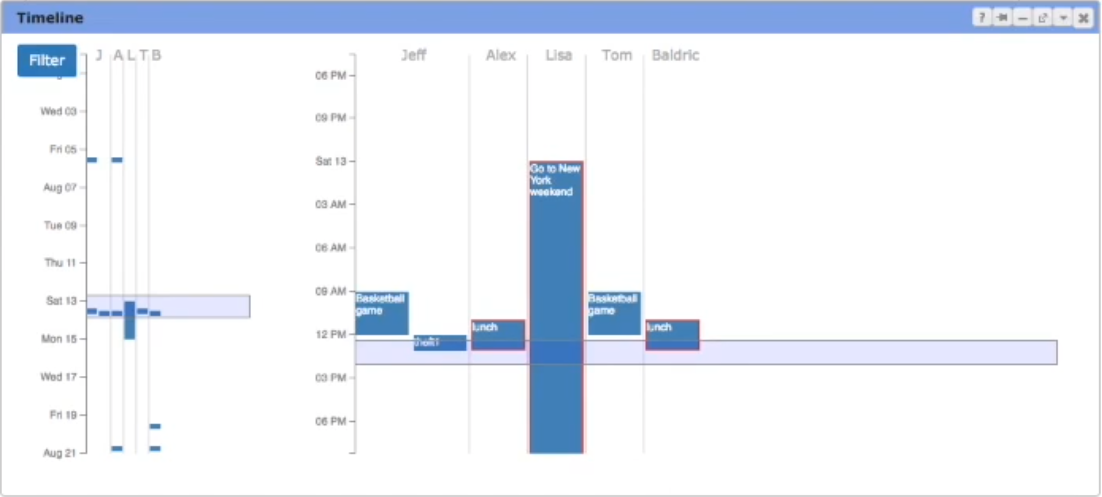
\includegraphics[width=\columnwidth]{03-System/img/timeline2.png}
	\caption{The improved timeline in CAnalytics V2 displays events schematized by people. Selection on the left overview panel zooms the view into a specific range of time. Selection on the right detailed view selects events that overlap with a time range and applies a filter to other views (e.g. map, table and network) to narrow down data relevant to the selected events. This tool helps find alibi of suspects and identify correlation of events/time with other pieces of information. \label{fig:timeline2}}
\end{figure}

\paragraph{Capability to restore deleted data}

In Study One we noticed that participants removed data that were not relevant to their hypothesis to reduce noise. For example, if they had excluded the possibility of a suspect, it made sense to remove the suspect from the visualizations. However, we found that it often happened that analysts refuted their hypotheses and rewound back to the original evidence. Going back and forth in the evidence is a frequent operation although analysts do not need all pieces of evidence all the time. 

In CAnalytics V2, instead of \emph{``deleting''} a data object, analysts can \emph{``archive'' } an object. Archived data are hidden in visualization such as the network and the map, but are still accessible in the data table. They were grayed out and ranked in the end, but were searchable and could be ``restored'' if needed. 

\paragraph{Animated change}

Another subtle improvement is adding animated change made by teammates. For example, when an analyst is deleting an object, collaborators can easily miss that person's intention to delete the object and even the deletion action itself. One design solution is to make small actions larger. In this case, we use animation to make the delete action more prominent. This could be done by adding a visual effect atop the deleted object to emphasize that it has been selected, and then adding an animation to the actual delete event to make it more salient, where it perhaps grows in size for a few seconds before shrinking to nothing \citep{Greenberg2001}. Similar animation is applied to adding a data object and editing an object.


\section{Use case demonstration}

To demonstrate the usage of the collaborative hypothesis development feature in CAnalytics V2, we run a use case in Table~\ref{tab:demo}. The full video is available at \url{https://youtu.be/pHqOukeg2KA}.

\begin{table}
	\caption{A demonstration of collaborative hypothesis development in CAnalytics V2}
	\label{tab:demo}
	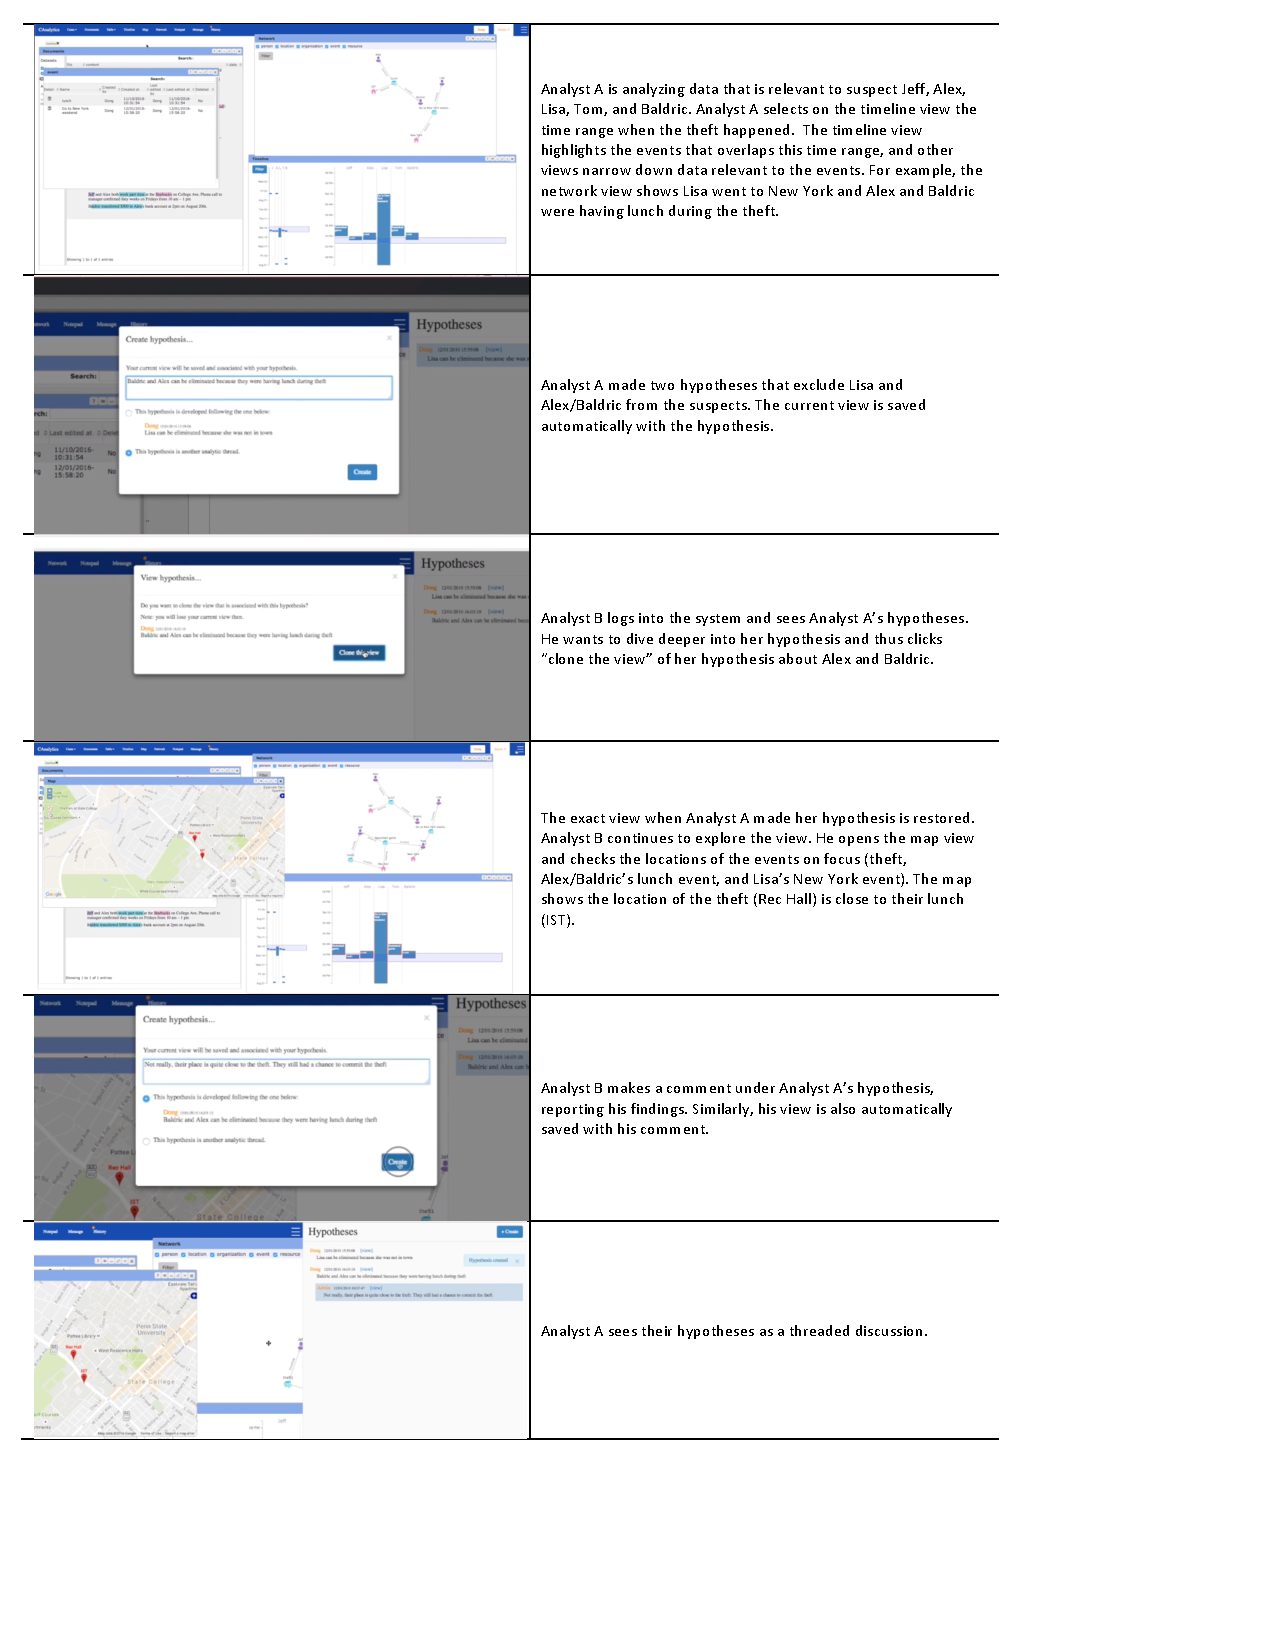
\includegraphics[width=1.2\columnwidth]{05-Study_two/img/demo.pdf}
\end{table}
